\documentclass[11pt,a4paper]{article}

\usepackage[utf8]{inputenc}
\usepackage[T1]{fontenc}
\usepackage[english]{babel}
\usepackage{graphicx}
\usepackage{booktabs}
\usepackage{amsmath,amssymb}
\usepackage{geometry}
\usepackage{hyperref}
\usepackage{caption}
\usepackage{subcaption}
\usepackage{siunitx}
\usepackage{enumitem}
\usepackage{float}

\geometry{margin=2.5cm}
\hypersetup{colorlinks=true,linkcolor=blue,urlcolor=blue,citecolor=blue}

\title{Robustness of Operating-Room Scheduling Metaheuristics\\under Length-of-Stay Uncertainty}
\author{Individual contribution --- Virna Lissi MARTÍNEZ SÁNCHEZ\\Centrale Lille, 7th semester, IA et Santé}
\date{\today}

\begin{document}
\maketitle

\begin{abstract}
\noindent
We evaluate five metaheuristics for operating-room scheduling under length-of-stay (LOS) uncertainty. Using an XGBoost LOS predictor (MAE = \SI{0.412}{days}, \(R^2 = 0.789\)) with 90\% split-conformal intervals (\(\pm \SI{1.02}{days}\)), we generate instances at small (\(n=45\)) and large (\(n=420\)) scales. At large scale, Simulated Annealing (SA), Tabu Search and the Tabu\(\times\)SA hybrid reach a cost of \(5198\)--\(5207\), within \(0.3\%\) of the lower bound (\(5190\)) imposed by unavoidable overrun in one specialty. The Genetic Algorithm (GA) with default hyperparameters (\(p_{\mathrm{mut}}=0.08\)) is misconfigured and reaches \(8569\); a sensitivity check shows that with \(p_{\mathrm{mut}}=1/n\), GA drops to \(5287\) and nearly matches the local-search methods. ACO reaches \(5783\) but is \(12\)--\(37\times\) slower than the others. Monte Carlo re-evaluation of frozen schedules on \(200\) LOS scenarios shows that schedules planned on the point prediction cost about \(2\%\) more under uncertainty, almost entirely through bed overrun: sampled stays are 0.2 days longer on average, pushing bed occupancy from about \(97\%\) to \(103\%\) of capacity. Planning on the conformal upper bound makes schedules much less sensitive to this shift (+6 to +17 instead of +109 to +115) and less dispersed, but raises the expected cost of SA, Tabu and the hybrid by 63--102 (paired differences of at least 4.9 standard errors). In this setting, the upper bound therefore buys predictability, not lower expected cost. 
\end{abstract}

\section{Introduction}
Operating-room scheduling is a combinatorial problem in which several scarce resources (rooms, surgeons, beds) must be coordinated simultaneously. Most metaheuristic benchmarks assume deterministic intervention and stay durations, ignoring the operational reality that LOS is uncertain. This work extends the group's \texttt{optimiseur/} package with LOS uncertainty from a predictive model and studies how schedules planned by five metaheuristics on predicted durations behave when actual stays differ from the prediction.

\section{Methods}

\subsection{Predictive LOS model}
\begin{itemize}[nosep]
  \item \textbf{Model:} XGBoost regressor trained on \(\log(1+\mathrm{LOS})\).
  \item \textbf{Test metrics:} MAE \(= \SI{0.412}{days}\), \(R^2 = 0.789\).
  \item \textbf{Uncertainty:} 90\% split-conformal interval, half-width \(\pm \SI{1.02}{days}\), empirical coverage \(89.4\%\).
  \item \textbf{Risk classifier:} long-stay threshold \(= \SI{4}{days}\); the HIGH category reaches a true long-stay rate of \(79.3\%\).
\end{itemize}

\subsection{Group optimizer}
Five metaheuristics from \texttt{optimiseur/optimizer.py}:
\begin{itemize}[nosep]
  \item \textbf{SA} (Recuit simul\'e)
  \item \textbf{Tabu} (Recherche Tabou)
  \item \textbf{GA} (Algorithme g\'en\'etique)
  \item \textbf{Hybrid} (Tabou \(\times\) Recuit)
  \item \textbf{ACO} (Colonie de fourmis)
\end{itemize}
The cost function is a weighted sum of vacation-capacity overrun (\(w=5\)), bed-capacity overrun (\(w=3\)), and load imbalance across vacations (\(w=0.05\)). We report cost directly (lower is better); a cost of \(0\) is a perfect schedule.

\subsection{The proposed bridge --- \texttt{bridge\_los.py}}
We extend the group's \texttt{data\_bridge.py} with LOS uncertainty. For each patient in the horizon-filtered EDA window:
\begin{itemize}[nosep]
  \item \texttt{duree\_sejour} = LOS point prediction;
  \item \texttt{duree\_sejour\_lower} / \texttt{duree\_sejour\_upper} = conformal 90\% interval;
  \item \texttt{risk\_level} = LOW / HIGH (threshold \(=4\) days).
\end{itemize}
The match rate on the EDA \(\to\) LOS join is \(86.7\%\) (small) and \(86.4\%\) (large). Unmatched rows fall back to the global median prediction.

\subsection{Experimental design}
\begin{itemize}[nosep]
  \item \textbf{Small:} horizon \(=5\) days \(\to\) \(45\) patients, \(35\) vacations.
  \item \textbf{Large:} horizon \(=30\) days \(\to\) \(420\) patients, \(210\) vacations.
  \item \textbf{Planning modes:} point LOS (nominal) and conformal upper bound (upper).
  \item \textbf{Seeds:} \(10\) (\(42\)--\(51\)).
  \item \textbf{Monte Carlo:} each schedule is planned once (on the point LOS or on the upper bound), then frozen and re-evaluated without re-optimizing on 200 LOS scenarios sampled uniformly within \(\pm 1.02\) days of the unrounded prediction (floored at 1 day), using the same scenarios for all methods. We report the mean, the 95th percentile and paired differences.
  \item \textbf{GA sensitivity:} one additional run with \(p_{\mathrm{mut}}=1/n\) (same seeds and scenarios).
\end{itemize}

\section{Results}

\subsection{Solution quality}
Figure~\ref{fig:cost} reports mean cost by method and planning mode.

\begin{figure}[H]
\centering
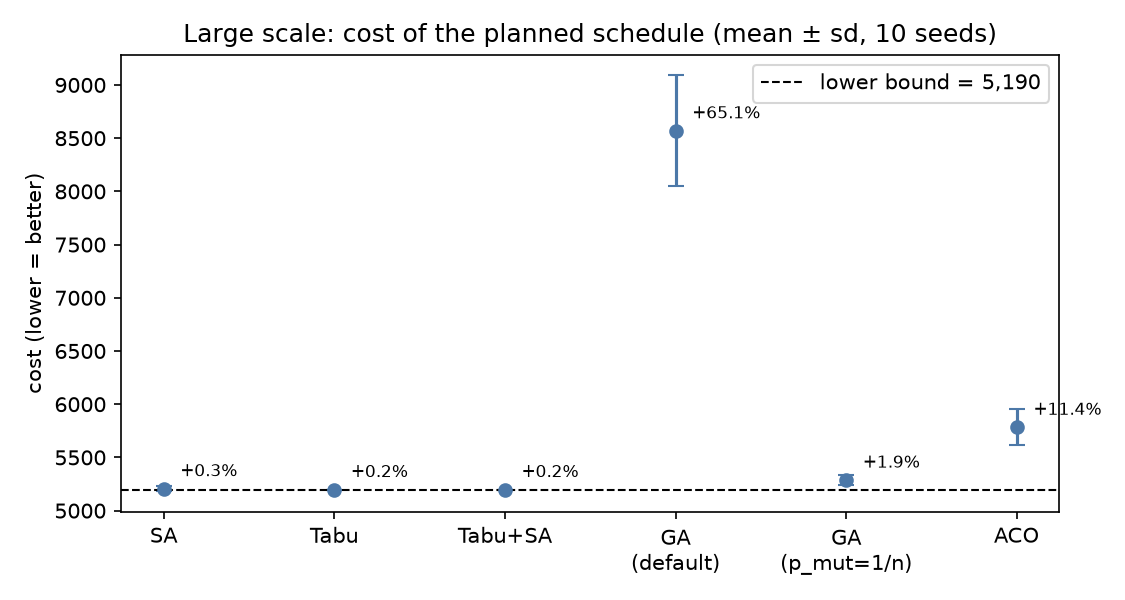
\includegraphics[width=\linewidth]{figures/fig1_cost_large.png}
\caption{Mean cost by method and planning mode, large scale (\(n=420\)). Lower is better.}
\label{fig:cost}
\end{figure}

\noindent\textbf{Small scale.} All five methods converge to nearly identical cost (\(3.25\)--\(3.29\)), against \(4.56\) for a random schedule. There is no overrun in operating-rooms or beds, so the cost reduces to the load-balance term and LOS sampling has no effect. The problem is too small to discriminate between methods.

\noindent\textbf{Large scale.} Table~\ref{tab:quality} reports mean cost over \(10\) seeds.

\begin{table}[H]
\centering
\caption{Large scale (\(n=420\)), schedules planned on point-prediction LOS; \(10\) seeds. Lower bound on cost: \(5190\) (\(= 5 \times 1038\) min of unavoidable overrun in one specialty, computed from \texttt{floor\_check.py}).}
\label{tab:quality}
\small
\setlength{\tabcolsep}{4pt}
\begin{tabular}{lccc}
\toprule
Method & {Cost (mean \(\pm\) sd)} & {Gap to bound (\%)} & {OR overrun (min)} \\
\midrule
SA                          & 5207 \(\pm\) 26     & +0.3   & 1040 \\
Tabu                        & 5198 \(\pm\) 0      & +0.2   & 1038 \\
Tabu\(\times\)SA            & 5198 \(\pm\) 0      & +0.2   & 1038 \\
GA (default)                & 8569 \(\pm\) 521    & +65.1  & 1696 \\
GA (\(p_{\mathrm{mut}}=1/n\)) & 5287 \(\pm\) 44   & +1.9   & 1047 \\
ACO                         & 5783 \(\pm\) 170    & +11.4  & 1146 \\
Random                      & 16848 \(\pm\) 2454  & +224.6 & 3339 \\
\bottomrule
\end{tabular}
\normalsize
\end{table}

The per-specialty lower bound from \texttt{floor\_check.py} is \(1038\) minutes of unavoidable overrun in specialty~N, giving a global lower bound on cost of \(5190\). Tabu and Tabu\(\times\)SA reach \(5198\) (gap \(+0.2\%\)) and SA \(5198\) \(+0.3\%\), i.e.\ essentially optimal in the dominant dimension. ACO reaches \(5783\) (gap \(+11.4\%\)). GA with default hyperparameters (\(p_{\mathrm{mut}}=0.08\)) reaches \(8569\) (gap \(+65.1\%\)), but is not intrinsically worse: a sensitivity sweep shows that with \(p_{\mathrm{mut}}=1/n\), GA drops to \(5287\) (gap \(+1.9\%\)), nearly matching SA/Tabu. It nevertheless remains \(89 \pm 17\) above SA in expected cost under LOS scenarios.

\subsection{Computation time}
Figure~\ref{fig:time} shows mean computation time on a logarithmic scale.

\begin{figure}[H]
\centering
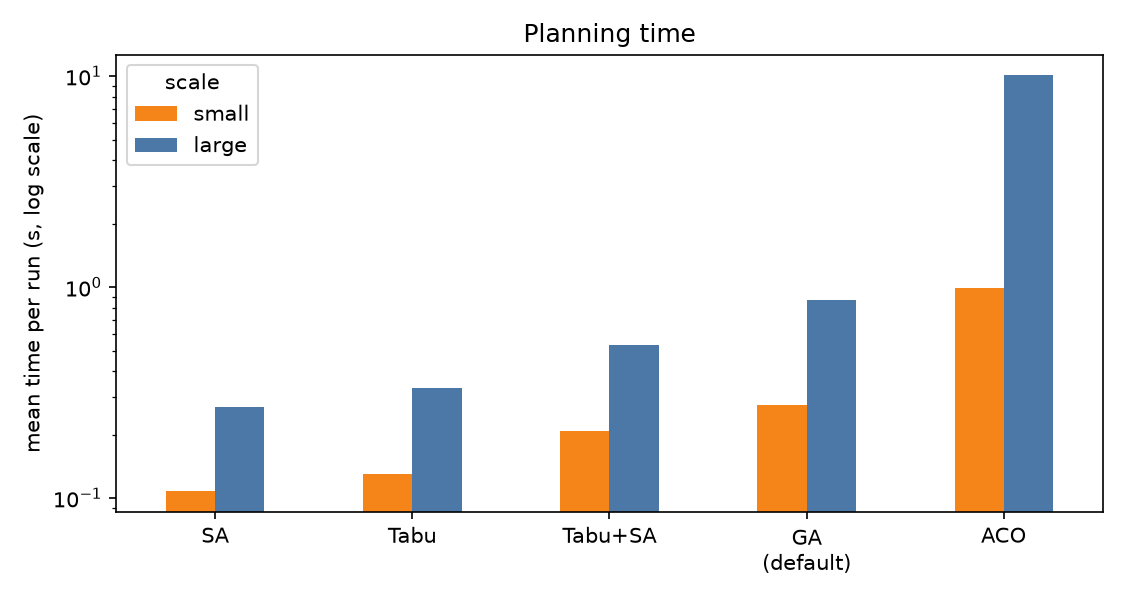
\includegraphics[width=0.9\linewidth]{figures/fig2_time.png}
\caption{Mean computation time by method and scale (log scale).}
\label{fig:time}
\end{figure}

\begin{table}[H]
\centering
\caption{Mean planning time per run (both planning modes, all seeds), default hyperparameters.}
\label{tab:time}
\begin{tabular}{lS[table-format=1.2]S[table-format=2.2]}
\toprule
Method & {Small (s)} & {Large (s)} \\
\midrule
SA            & 0.11 & 0.27 \\
Tabu          & 0.13 & 0.33 \\
Tabu\(\times\)SA & 0.21 & 0.53 \\
GA            & 0.28 & 0.87 \\
ACO           & 0.99 & 10.08 \\
\bottomrule
\end{tabular}
\end{table}

ACO is the slowest: at large scale it requires \(10.08\)~s, versus \(0.27\)~s for SA (\(37\times\) slower), \(0.33\)~s for Tabu, \(0.53\)~s for the hybrid, and \(0.87\)~s for GA (\(12\times\) slower).

\subsection{Robustness to LOS uncertainty (Monte Carlo)}
Figure~\ref{fig:robust} reports the Monte Carlo re-evaluation of frozen schedules on \(200\) LOS scenarios.

\begin{figure}[H]
\centering
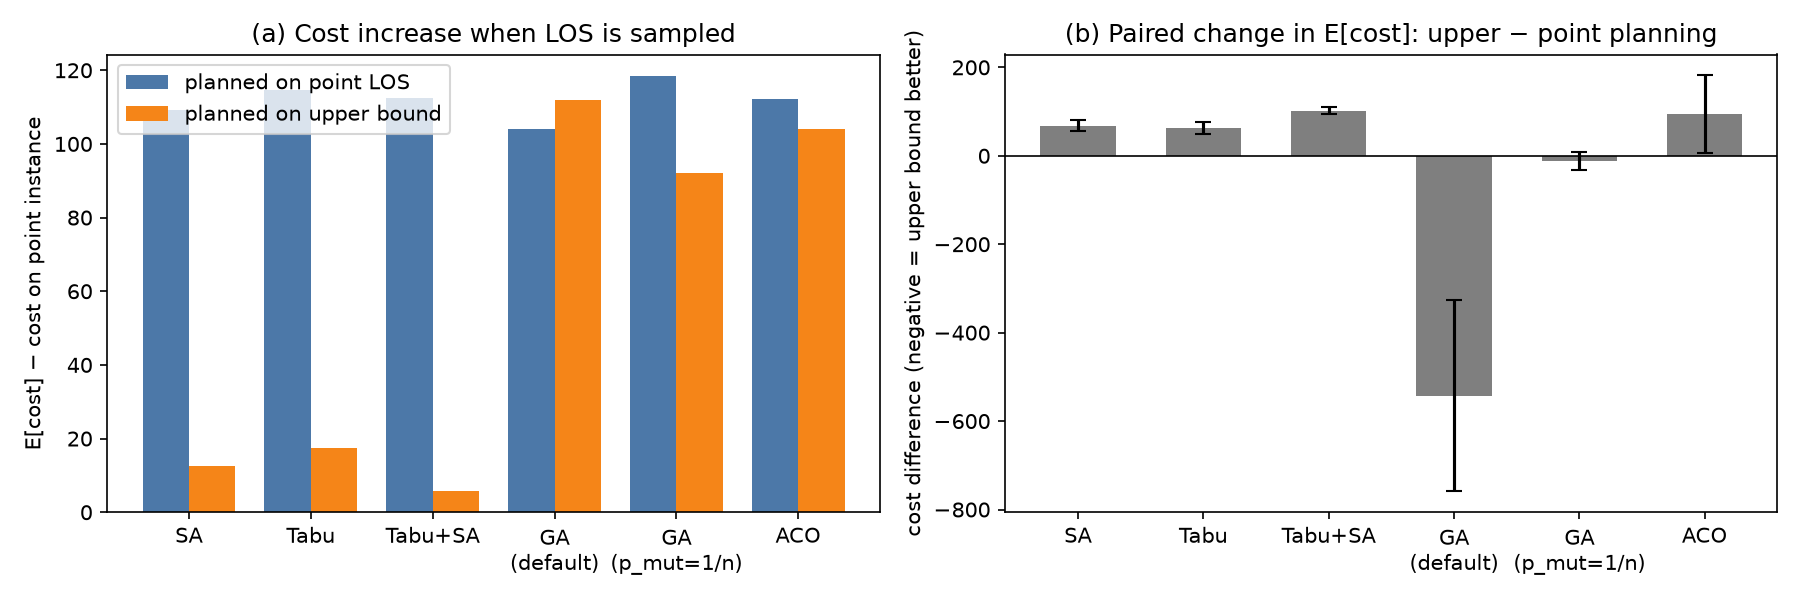
\includegraphics[width=0.9\linewidth]{figures/fig3_robustness.png}
\caption{Monte Carlo robustness: expected cost under \(200\) sampled LOS scenarios, for schedules planned on the point prediction (blue) and on the conformal upper bound (red).}
\label{fig:robust}
\end{figure}

\begin{table}[H]
\centering
\caption{Large scale. Frozen schedules re-evaluated on \(200\) LOS scenarios drawn from the 90\% conformal interval; \(10\) seeds. E[cost] is the mean cost over scenarios; Increase is E[cost] minus the cost on the point-prediction instance; the last column is the paired difference in E[cost] (mean \(\pm\) standard error over seeds).}
\label{tab:robust}
\small
\setlength{\tabcolsep}{4pt}
\begin{tabular}{lccccc}
\toprule
 & \multicolumn{2}{c}{Planned on point LOS} & \multicolumn{2}{c}{Planned on upper bound} & {Paired \(\Delta\)} \\
\cmidrule(lr){2-3} \cmidrule(lr){4-5}
{Method} & {E[cost]} & {Increase} & {E[cost]} & {Increase} & {(upper \(-\) point)} \\
\midrule
SA                          & 5316 & +109 & 5384 & +13  & \(+68 \pm 12\) \\
Tabu                        & 5313 & +115 & 5376 & +17  & \(+63 \pm 13\) \\
Tabu\(\times\)SA            & 5311 & +112 & 5413 & +6   & \(+102 \pm 8\) \\
GA (default)                & 8673 & +104 & 8131 & +112 & \(-542 \pm 217\) \\
GA (\(p_{\mathrm{mut}}=1/n\)) & 5405 & +118 & 5393 & +92  & \(-12 \pm 20\) \\
ACO                         & 5896 & +112 & 5990 & +104 & \(+94 \pm 88\) \\
\bottomrule
\end{tabular}
\normalsize
\end{table}

Schedules planned on the point prediction increase by roughly the same amount (\(+104\) to \(+118\), about \(2\%\)) when LOS is sampled, regardless of the method. This increase comes entirely from the bed term: sampled LOS averages \(2.10\) days versus \(1.90\) for the point prediction, increasing bed-days from about \(1219\) to \(1301\) against a capacity of \(1260\). Planning on the conformal upper bound reduces the increase to \(+13\) (SA), \(+17\) (Tabu) and \(+6\) (Tabu\(\times\)SA), but these schedules start from worse point-prediction costs (\(5372\), \(5359\) and \(5407\) versus \(5207\), \(5198\) and \(5198\)). Their expected cost is also higher: the paired difference (upper \(-\) point) is \(+68 \pm 12\) (SA), \(+63 \pm 13\) (Tabu) and \(+102 \pm 8\) (Tabu\(\times\)SA). Their 95th percentile is higher by \(43\)--\(76\), although the spread of outcomes (\(p95\) minus mean) shrinks from about \(38\) to \(12\)--\(17\). GA with default hyperparameters behaves differently (\(-542 \pm 217\)), although it remains about \(53\%\) above SA; with \(p_{\mathrm{mut}}=1/n\), the effect is not detectable (\(-12 \pm 20\)). ACO's paired difference is inconclusive (\(+94 \pm 88\)).

\clearpage
\section{Discussion}

\paragraph{Quality: local-search methods reach the lower bound.}
SA, Tabu and Tabu\(\times\)SA are not mediocre: they reach a cost of \(5198\), within \(0.3\%\) of the theoretical lower bound \(5190\) imposed by unavoidable overrun in specialty~N. GA with default hyperparameters is misconfigured; a single change (\(p_{\mathrm{mut}}=1/n\)) brings it to \(5287\), close to the local-search methods. The relevant comparison is therefore not ``GA vs.\ SA'' but ``well-configured GA vs.\ SA vs.\ Tabu'', all within \(2\%\) of each other in absolute cost.

\paragraph{Robustness: planning on the upper bound is the key lever.}
Planning on the upper bound anticipates longer stays, so its schedules react little when stays are sampled (\(+6\) to \(+17\)) and their outcomes are less dispersed. However, they start from a worse point and their expected cost remains \(1.2\)--\(1.9\%\) higher than that of schedules planned on the point prediction. The upper bound also overestimates its own cost (SA: planned \(5766\), expected \(5384\)). The choice of planning duration is therefore a trade-off rather than a free improvement. More importantly, LOS affects only the bed term, making all methods similarly sensitive to its variation.

\paragraph{Time considerations.}
ACO is \(12\times\) slower than GA and \(37\times\) slower than SA at large scale, for a worse absolute cost. SA is the fastest method and is within \(0.3\%\) of the lower bound. GA with default hyperparameters is neither fast nor good; with \(p_{\mathrm{mut}}=1/n\) it becomes competitive but still slower than SA/Tabu.

\paragraph{Operational recommendation.}
For a hospital deploying this scheduler under LOS uncertainty, we recommend:
\begin{itemize}[nosep]
\item \textbf{SA as the default planner} (0.27 s, within \(0.3\%\) of the lower bound), with \textbf{Tabu as an equivalent alternative}, planning on the point-prediction LOS;
\item \textbf{Planning on the conformal upper bound} only if lower outcome variability is valued more than a \(1.2\)--\(1.9\%\) higher expected cost;
\item \textbf{GA with \(p_{\mathrm{mut}}=1/n\)} as a second option (it remains \(89 \pm 17\) above SA in expected cost);
\item \textbf{ACO and the Tabu\(\times\)SA hybrid are not recommended}: ACO because of its \(10\) s runtime and \(11\%\) gap to the bound; the hybrid because it doubles SA's runtime without improving on Tabu.
\end{itemize}


\section{Limitations}
\begin{itemize}[nosep]
  \item Uniform sampling within the conformal interval underestimates the tails; the interval has constant width and is not heteroscedastic.
  \item Individual sprint; \(10\) seeds and \(2\) scales, without confidence intervals on all reported quantities.
  \item \textbf{LOS enters the cost only through the bed term} (about \(2\%\) of total cost) and bed capacity is fixed at \(42\) (\(\approx 97\%\) nominal utilization); this limits the power to discriminate methods on robustness; 
  \item \textbf{Sampled stays are floored at 1 day}, which raises mean LOS from \(1.90\) to \(2.10\) days (large scale); the reported cost increase mostly reflects this shift rather than variance; 
  \item \textbf{Only GA's mutation rate was tuned} (one alternative value); the other methods use default hyperparameters, so comparisons favor tuned GA over ACO; 
  \item \textbf{Bed occupancy is truncated at the end of the horizon}; schedules planned on the upper bound place more patients in the last 5 days (\(23\%\)--\(26\%\) vs. \(17\%\)), consistent with partly exploiting this truncation; 
  \item \textbf{The lower bound (\(5190\))} comes from the overload of one specialty (demand \(15{,}438\) min vs. capacity \(14{,}400\) min) under the group's model of one \(480\)-min vacation per specialty per day; it makes the large instance easy for local search;
  \item \texttt{risk\_level} is a threshold (4 days) on the regression output, not the classifier of Section 2.1. 
  \item The LOS \(\to\) EDA join leaves \(\sim 14\%\) of rows unmatched, falling back to the global median.
  \item No integration with the ongoing SMA (\texttt{hospital\_sim/}) --- coordinated future work.
\end{itemize}

\section{Conclusion}

This work addressed the gap between predictive modeling and scheduling optimization in operating-room management. We proposed \texttt{bridge\_los.py}, a reusable bridge that injects LOS uncertainty from an XGBoost predictive model into the group's metaheuristic scheduler. The bridge achieves an \(86.7\%\) match rate on real EDA data and produces per-patient duration predictions with conformal 90\% intervals and risk levels.

Our experimental evaluation compared five metaheuristics at small and large scales, under both point-prediction planning and conformal-upper-bound planning, with Monte Carlo re-evaluation on \(200\) sampled LOS scenarios. The results reveal a clear picture:

\begin{itemize}
  \item \textbf{Best absolute quality: SA, Tabu and Tabu\(\times\)SA.} At large scale, they reach a cost of \(\approx 5198\), within \(0.3\%\) of the theoretical lower bound \(5190\). GA with default hyperparameters is misconfigured (\(8569\)); with \(p_{\mathrm{mut}}=1/n\), it drops to \(5287\) and becomes competitive.
  \item \textbf{Robustness: the upper bound trades expected cost for predictability.} Planning on the conformal upper bound makes schedules less sensitive to LOS scenarios (\(+6\) to \(+17\) instead of \(+109\) to \(+115\)) but increases expected cost by \(63\)--\(102\) (\(1.2\)--\(1.9\%\)). The observed increase is mostly a mean shift (\(+0.2\) days) acting on the bed term, which accounts for about \(2\%\) of the total cost, so robustness differences between methods remain small.
  % \item \textbf{Best time--quality compromise: SA.} SA runs in \(0.27\)~s at large scale and reaches the lower bound. ACO requires \(10.08\)~s and is not recommended.
\end{itemize}

\paragraph{Recommendation.} For real hospital deployment, \textbf{SA (or Tabu) planned on the point-prediction LOS} is the default choice. The conformal upper bound can be used as the planning duration when outcome predictability matters more than expected cost. \textbf{GA with \(p_{\mathrm{mut}}=1/n\)} is a viable alternative if population-based exploration is desired. \textbf{ACO and the Tabu\(\times\)SA hybrid are not recommended.}

The bridge is directly reusable by the SMA workstream (\texttt{hospital\_sim/}) and can be extended with asymmetric conformal intervals as future work.

\begin{thebibliography}{3}

\bibitem{xgb}
T.~Chen and C.~Guestrin, ``XGBoost: A Scalable Tree Boosting System,''
\emph{Proceedings of the 22nd ACM SIGKDD International Conference on Knowledge Discovery and Data Mining (KDD '16)}, 2016, pp.~785--794.
\url{https://doi.org/10.1145/2939672.2939785}

\bibitem{cp}
H.~Papadopoulos, K.~Proedrou, V.~Vovk, and A.~Gammerman, ``Inductive Confidence Machines for Regression,''
\emph{Machine Learning: ECML 2002}, Lecture Notes in Computer Science, vol.~2430, Springer, 2002, pp.~345--356.
\url{https://doi.org/10.1007/3-540-36755-1_29}

\bibitem{tabu}
F.~Glover, ``Tabu Search---Part I,''
\emph{ORSA Journal on Computing}, vol.~1, no.~3, pp.~190--206, 1989.
\url{https://doi.org/10.1287/ijoc.1.3.190}

\end{thebibliography}

\end{document}